\documentclass[12pt,UTF8]{ctexbook}
\usepackage{ctex}
\usepackage{caption}
\usepackage{graphicx}
\usepackage{float}
\usepackage{wrapfig}
\usepackage{array}
\usepackage[table, dvipsnames, svgnames, x11names]{xcolor}
\usepackage{colortbl}% 
\usepackage{tabularx}
\usepackage{amsmath, tikz}
\usepackage{amssymb}
\usepackage{xfrac}
\usepackage{eucal}
\usepackage{titlesec}
\usepackage{amsthm}
\usepackage{ifthen}
\usepackage{tikz-cd}
\usepackage{enumitem}
\usepackage{verbatim}
\usepackage{fontspec,xunicode,xltxtra}
\usepackage{xeCJK} 

\definecolor{gl}{RGB}{246, 252, 240}
\definecolor{gd}{RGB}{236, 244, 230}
\definecolor{bg}{RGB}{242, 244, 228}


\setCJKmainfont[BoldFont=STZhongsong]{STSong}
\setCJKmonofont{simkai.ttf} % for \texttt
\setCJKsansfont{simfang.ttf} % for \textsf
\setlength\parskip{8pt}
\setlength{\fboxsep}{12pt}
\renewcommand\thesection{\arabic{chapter}.\arabic{section}}

\usetikzlibrary{calc,topaths}

\newcommand\widearc[1]{%
    \tikz[baseline=(wideArcAnchor.base)]{
        \node[inner sep=0] (wideArcAnchor) {$#1$}; 
        \coordinate (wideArcAnchorA) at ($(wideArcAnchor.north west) + (0.15em,0.1em)$);
        \coordinate (wideArcAnchorB) at ($(wideArcAnchor.north east) + (0.0em,0.1em)$);
    %
        \draw[line width=0.1ex,line cap=round,out=45,in=135] (wideArcAnchorA) to (wideArcAnchorB);
    }
}

% \newcommand{\jch}[2][]{
%     \begin{tikzpicture}[baseline]
%         \draw (-0.16em,0.32em) -- (0em,0.32em) -- (0em,-0.2em) -- (1em,-0.2em);  
%         \ifthenelse{\equal{$#1$}{}}{\node at (0.5em,0.3em) {$#1$}}{\node at (0.5em,0.3em) {$#2$}};
%         \ifthenelse{\equal{$#1$}{}}{}{\node at (0em,0.56em) {$\scriptscriptstyle #1$}};
%     \end{tikzpicture}
% }
\newtheorem{df}{定义}[section] 
\newtheorem{pp}{命题}[section]
\newtheorem{tm}{定理}[section]
\newtheorem{ex}{例子}[section]
\newtheorem{sk}{思考}[section]
\newtheorem{po}{公理}
\newtheorem*{so}{解答}
\newtheorem*{proof2}{证明}
\newtheorem{xt}{习题}[section]
\newtheorem{cor}{推论}[pp]
\renewcommand{\proofname}{\indent\bf 证明}
\renewcommand{\qedsymbol}{\hfill$\square$}
% 列举环境的行间距
\setenumerate[1]{itemsep=0pt,partopsep=0pt,parsep=0pt,topsep=0pt}
\setitemize[1]{itemsep=0pt,partopsep=0pt,parsep=0pt,topsep=0pt}
\setdescription{itemsep=0pt,partopsep=0pt,parsep=0pt,topsep=0pt}
\setlength{\intextsep}{2pt}%
\setlength{\columnsep}{2pt}%
% 新函数
\renewcommand\parallel{\mathrel{/\mskip-4mu/}}
% 章节字体大小
\titleformat{\section}{\zihao{-2}\bfseries}{ \thesection }{16pt}{}
% 封面
\title{\zihao{0} \bfseries 第五册}
\author{\zihao{2} \texttt{大青花鱼}}
% \date{\bfseries\today}
\date{}
% 正文
\begin{document}
\maketitle
\tableofcontents
\newpage

\chapter{圆}

学习反比例函数和二次函数时,我们发现,就算是简单代数式定义的函数,它的图像也是我们无法手动画出的曲线。
曲线是比直线更复杂的形状。为了给我们今后研究各种曲线打下基础,以下我们研究一种简单的曲线:圆。

\section{圆的基本性质}
我们已经学过圆的概念。公理体系中,我们这样定义圆:平面上到定点$O$距离为定长的点的集合,是一个圆。
给定线段$XY$,到$O$的距离和$AB$等长的点构成一个圆。$O$叫做\textbf{圆心},
$XY$叫做圆的\textbf{半径},长度一般记为$r$。不至于混淆的时候,半径的长也简称为半径。

圆心为$O$、半径为$r$的圆,一般记为圆$(O, r)$或$\odot_{(O, r)}$。
圆心$O$和另一点$P$确定的圆,一般记为圆$(O, P)$或$\odot_{(O, P)}$。如果不在意半径,在不至于混淆的情况下,
也可以简记为圆$O$。

平面上的点到$O$的距离小于$r$,就说它在圆内;如果等于$r$,就说它在圆上;如果大于$r$,就说它在圆外。

和引进直线等概念时一样,圆也有一条公理,规定它和直线的关系。
\begin{po}\textbf{直线交圆公理}\label{po:0}
    直线和圆有两个交点,当且仅当直线有部分在圆内。
\end{po}

从这个公理出发,我们可以整理直线和圆的位置关系。

考虑直线$l$和圆$\odot_{(O, r)}$。过$O$作直线$m\perp l$,记垂足为$P$,$|OP| = d$。

\begin{figure}[h] %this figure will be at the right
    \vspace{8pt}
    \centering
    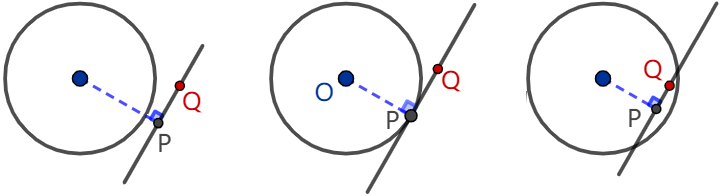
\includegraphics[width=0.72\textwidth]{圆与直线1.png}
\end{figure}

\begin{enumerate}
    \item 如果$d > r$,那么$P$在圆外。根据垂距定理,$l$上任意点都在圆外。我们说直线$l$与圆$O$\textbf{相离}。反之,如果直线与圆相离,那么$P$在圆外,因此$d > r$。
    \item 如果$d = r$,那么$P$在圆上。根据垂距定理,$l$上的点除了$P$都在圆外。直线和圆恰有一个公共点。我们说直线$l$与圆$O$\textbf{相切},称$P$为\textbf{切点}。
    反之,如果直线与圆相切于点$Q$,那么$|OQ| = r$。$l$上其他点都在在圆外,所以根据垂距定理的逆定理,$OQ \perp l$,$d = r$。
    \item 如果$d < r$,那么$P$在圆内。根据直线交圆公理,直线和圆有两个交点$A$、$B$。我们说直线与圆\textbf{相交},或直线\textbf{割圆}于$A$、$B$。
    反之,如果直线和圆有两个交点,那么根据直线交圆公理,直线有部分在圆内,这部分上的点到圆心距离小于$r$,因此根据垂距定理,$d < r$。
\end{enumerate}

设直线割圆于两点$A$、$B$,我们说直线是圆的\textbf{割线}。根据直线交圆公理,线段$AB$(除端点)在圆内。
我们把线段$AB$称为圆的一条\textbf{弦}。如果$AB$过圆心$O$,就说它是圆的直径,$A$、$B$互为\textbf{对径点}。
直径是过圆心的弦。它的长度是半径的两倍。不至于混淆的时候,直径的长也简称为直径。

考虑圆$O$上的弦$AB$的垂直平分线$m$,圆心$O$显然在$m$上。$m \perp AB$,设垂足为$P$,那么$|AP| = |PB|$。
设$m$和圆交于两点$C,D$,则弦$CD$就是直径。所以我们说:\textbf{恰有一条直径平分每条弦}。


% 考虑两个圆:$\odot_{(O_1, r_1)}$和$\odot_{(O_2, r_2)}$,设两个圆心的距离是:$|O_1O_2| = s$,
% 那么,两个圆的关系可能有以下几种:

% \begin{figure}[h] %this figure will be at the right
%     \vspace{8pt}
%     \centering
%     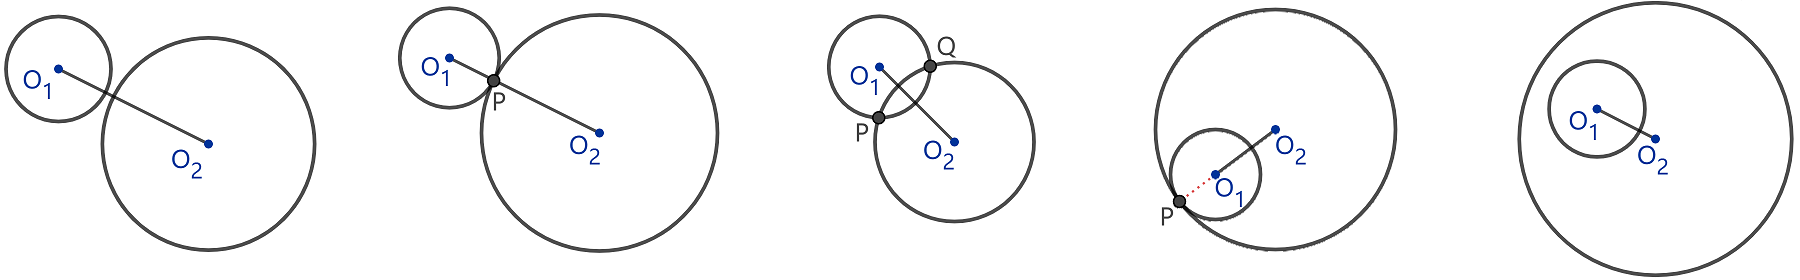
\includegraphics[width=0.9\textwidth]{圆与圆1.png}
% \end{figure}

% \begin{enumerate}
%     \item $s > r_1 + r_2.$ 用反证法可以证明,两个圆没有公共点。我们说两圆\textbf{相离}。
%     \item $s = r_1 + r_2.$ 考虑线段$O_1O_2$,上面有一点$P$使得$|O_1P| = r_1$,于是$|PO_2| = |O_1O_2| - |O_1P| = r_2$。
%     这说明两个圆有一个公共点。如果点$Q$不在线段$O_1O_2$上,则$|O_1Q| + |QO_2| > |O_1O_2|$。
%     于是$Q$不可能是公共点。也就是说,两个圆恰有一个共同点,在圆心连线上。我们说两圆\textbf{外切}。
%     \item $|r_1 - r_2| < s < r_1 + r_2.$ 根据第二个公理,$\odot_{(O_1, r_1)}$和$\odot_{(O_2, r_2)}$恰有两个公共点,分别在圆心连线两侧。我们说两圆\textbf{相交}。
%     \item $s = |r_1 - r_2|.$ $r_1 > r_2$时,$s = r_1 - r_2$。考虑直线$O_1O_2$,上面有一点$P$,使得$|O_1P| = r_1$,且和$O_2$在$O_1$同一边。于是$|O_2P| = |O_1P| - |O_1O_2| = r_2$。
%     这说明两个圆有一个公共点。如果点$Q$不在线段$O_1O_2$上,则$|O_1O_2| + |QO_2| < |O_1Q|$。
%     于是$Q$不可能是公共点。也就是说,两个圆恰有一个共同点,在圆心连线上。$r_1 > r_2$时,通过类似推理可以得到同样的结论。我们说两圆\textbf{内切}。
%     \item $s < |r_1 - r_2|.$ 用反证法可以证明,两个圆没有公共点。如果$r_1 > r_2$,我们说$\odot_{(O_1, r_1)}$\textbf{内含}$\odot_{(O_2, r_2)}$,$\odot_{(O_2, r_2)}$\textbf{内含于}$\odot_{(O_1, r_1)}$;反之亦然。
% \end{enumerate}
% 要注意的是,如果仅知道两圆恰有一个公共点,我们无法判断到底是第二还是第四种情形;如果仅知道两圆没有公共点,我们无法判断到底是第一还是第五种情形。
% 第二和第四种情形可以统称为两圆\textbf{相切},第一和第五种情形可以统称为两圆\textbf{相离}。
    % \indent 2. 完成两圆关系的第一和第五种情形中的证明。\\
    % \indent 3. 阐明两圆关系的第四种情形中,$r_1 > r_2$情况下的推理过程。

\begin{xt}\label{xt:0-0-0}
    补充:\\
    \indent 1. 设直线割圆于两点$A$、$B$,证明线段$AB$(除端点)在圆内。\\
    \indent 2. 证明:同一个圆中,直径是最长的弦。
\end{xt}

\section{圆和旋转}
怎么画一个圆?我们用圆规画圆。如果已知圆心和圆上一点,我们将圆规尖定在要画的圆心处,
将笔头接触圆上的点,然后轻轻旋转,笔头就画出一个圆。如果已知圆心和半径线段,我们首先张开圆规,
圆规尖和笔头分别对齐半径两端,然后保持圆规形状不变,将圆规尖定在要画的圆心处,让笔头接触纸面,
轻轻旋转,笔头就画出一个圆。

可以看出,圆和旋转有天然的关系。旋转是由角定义的操作,把平面中的点映射到另一点。
给定角$AOB$,可以这样定义\textbf{旋转}:

\begin{df}\label{df:0-1-0}
    给定角$AOB$,平面中一点$P$关于$\angle AOB$旋转的结果,
    是唯一使得$\angle POQ = \angle AOB$且$|OP| = |OQ|$的点$Q$。
\end{df}
$O$称为旋转的\textbf{中心}。任何点$P$绕中心旋转,结果都在圆$(O,P)$上。

可以看到,给定一个圆$(O,P)$,从点$P$出发,旋转不同的角度,
就得到圆上其它的点。用圆规画圆时,从零角出发,随着角度不断增大,直到周角,我们沿逆时针经历了圆上所有的点
(注意:这里约定角度的范围是$0^\circ$到$369^\circ$)。
也就是说,我们认为零角到周角的角按角度和圆上的点之间有一一映射。
换句话说,数轴上$0$和$360$之间的数,和圆上的点之间有一一映射。
我们把它称作\textbf{圆映射},记为$\gamma_{(O,P)}$。

通过$\gamma_{(O,P)}$,我们可以把对圆的研究,改为对数轴上线段的研究。
这样就把曲线上的问题转为了直线上的问题。
比如,既然$[0, 360)$对应整个圆,那么$[0,180]$就对应半个圆,
$[0,60]$就对应六分之一个圆,等等。我们把闭区间对应的圆的部分称为\textbf{圆弧}。

同一圆上两个圆弧分别对应$[\, a_1, a_1+x\, ]$和$[\, a_2, a_2+x \,]$,这两个圆弧有什么不同吗?
观察圆的图像可知,并没有不同。也就是说,圆弧的形状只和它对应数轴上区间的长度有关,和它所在的位置无关。
只要对应的区间一样长,那么圆弧就全等,可以相互覆盖。换句话说,圆弧只要等长,就是全等的。
于是,线段所满足的公理,对同一个圆上的圆弧也成立。

和线段一样,圆弧也有起点和终点。比如$[\, 0,60\, ]$对应的圆弧,起点就是$P$,
终点是$60$度角$POQ$的终边和圆的交点$Q$。如果圆弧对应的区间长度超过$180$,就说它是\textbf{优弧};
如果圆弧对应的区间长度小于$180$,就说它是\textbf{劣弧};如果等于$180$,就说它是\textbf{半圆}。
优弧比半圆长,劣弧比半圆短。

从直线和圆相交的角度来看,圆上两点确定的直线将圆分为两个圆弧。这两个圆弧并起来就是圆,
所以要么一个是优弧、一个是劣弧,要么两者都是半圆(这时直线过圆心)。我们说它们互为\textbf{补弧}。

同一个圆上,明确了起点$A$和终点$B$,就唯一确定了圆弧$\widearc{AB}$。如果只说了两点$A$、$B$,
那么$\widearc{AB}$一般指劣弧或起点为$A$终点为$B$的圆弧。

\begin{xt}\label{xt:0-1-0}
    证明:\\
    \indent 1. 任意线段经过旋转得到等长的线段。\\
    \indent 2. 任意三角形经过旋转得到同角全等的三角形。 
\end{xt}

\section{圆心角和圆周角}

根据圆映射的定义,每个圆弧都对应一个顶点在圆心,大小介于零角和周角之间的角,称为它的\textbf{圆心角}。
圆弧还可以对应另一类角。给定起点为$A$,终点为$B$的圆弧$\widearc{AB}$和圆上弧外一点$P$,
则角$APB$称为一个\textbf{圆周角}。
每个圆弧只对应一个圆心角,但可以对应很多个圆周角。

同一段圆弧的圆心角和圆周角之间,有什么关系呢?如右图,连接$PO$,延长交圆于对径点$Q$。
由于$\triangle AOP$是等腰三角形,$\angle OAP + \angle OPA = 0$,
同理,$\angle OBP + \angle OPB = 0$。于是
\begin{align}
    \angle AOB &= \angle AOQ + \angle QOB \notag \\ 
    &= \angle OAP + \angle APO + \angle PBO + \angle OPB \notag \\
    &= 2\angle APO + 2\angle OPB = 2\angle APB \notag
\end{align}
也就是说,圆心角是圆周角的两倍大小,圆周角是圆心角的一半大小。

\begin{tm}\textbf{圆周角定理}\label{tm:0-2-0}
    给定圆$O$上的弧$\widearc{AB}$及圆上弧外的点$P$,如果$P \notin \widearc{AB}$,那么:
    $$\angle APB = \frac{1}{2} \angle AOB,$$
\end{tm}

如果点$P$在弧上,$\angle APB$和$\angle AOB$是什么关系呢?
这时$\angle APB$对应$\widearc{AB}$的补弧,于是它
是$\widearc{AB}$对应的圆心角的一半大小。$\widearc{AB}$对应的圆心角是周角减去$\angle AOB$,所以
$$\angle APB = 180^\circ - \frac{1}{2} \angle AOB.$$

对径点和圆心形成平角,因此,根据圆周角定理,对径点对应的圆周角是直角。或者说,半圆对应的圆周角是直角。

要注意的是,讨论圆心角时,我们约定角的范围是零角到周角。讨论圆周角和其他角时,为了方便,我们会切换到
负平角到正平角的范围。

同一个圆里,圆上的点$A$、$B$对应的圆心角$\angle AOB$和点$C$、$D$对应的圆心角$\angle COD$相等,那么
根据“边角边”,圆心$O$和它们构成的三角形满足:$\triangle AOB \simeq \triangle COD$。弦$AB$和$CD$也等长。
不仅如此,根据圆映射,圆弧$\widearc{AB}$和$\widearc{CD}$也等长。
事实上,$\widearc{CD}$就是$\widearc{AB}$关于某个角旋转的结果。
我们把这个结论称为“等角对等弦”、“等角对等弧”。

反之,如果两个圆弧$\widearc{AB}$和$\widearc{CD}$等长,那么它们对应的区间也一样长。
这说明它们对应的圆心角一样大。
圆心角既然相等,那么弦$AB$和$CD$也等长。
更进一步,设$P$是圆上不属于两弧的点,那么圆周角$\angle APB$和$\angle CPD$一样大。我们把这个结论称为“等弧对等弦”、“等弧对等角”。

反过来,如果圆$O$上两条弦$AB$和$CD$等长,那么根据“边边边”,$\triangle AOB \simeq \triangle COD$。
于是圆心角相等,所以劣弧$\widearc{AB}$和$\widearc{CD}$等长。我们把这个结论称为“等弦对等角”、“等弦对等弧”。

总的来说,在同一个圆里,两点对应的弦长相等当且仅当对应的(劣弧)弧长相等,当且仅当对应的圆心角相等,
当且仅当对应的圆周角相等。弦、弧、圆心角、圆周角,都是用来描述圆的部分和整体关系的方法。

给定圆上两点$A$、$B$,它们对应的垂直平分线$l$平分$\angle AOB$,即把$\angle AOB$分成两个相同大小的圆心角。
因此,设$l$和圆交于$P$、$Q$,则它们也分别平分所在的圆弧(称为弧的中点)。
我们把这一系列结论总称为垂径定理:
\begin{tm}\textbf{垂径定理 }\label{tm:0-2-1}
    给定圆上两点,则恰有圆的一条直径垂直平分两点对应的弦,同时平分对应的圆心角和两个圆弧。
\end{tm}
垂径定理也可以说成:过圆$O$的弦$AB$中点的直径与弦$AB$垂直,同时平分$\angle AOB$和弧$\widearc{AB}$。

给定圆$(O, r)$,弦$AB$中点记为$M$,$|MO|$称为弦$AB$的\textbf{弦心距}。由于$MO \perp AB$,
$\triangle OAM$是直角三角形,根据勾股定理,
$$|OM|^2 + |AM|^2 = |OA|^2 = r^2.$$
设直线$MO$与圆$O$交于$P$、$Q$两点,则
$$|MP| \cdot |MQ| = (r - |OM|)(r + |OM|) = r^2 - |OM|^2.$$
比较以上两式,可以得到:
$$ |MA| \cdot |MB| = |MA|^2 = |MB|^2 = |MP| \cdot |MQ|.$$
这个推论也常常被称为垂径定理。

\section{点到圆的势}
圆是到定点距离相同的点的集合,所以点对圆来说是关键的概念。
一点和圆的关系,可以用它到圆的距离来理解。点$P$在圆$(O, r)$上,当且仅当它到圆心的距离为$r$。

如果不知道圆心的位置,有没有办法理解点和圆的位置关系呢?
我们引进点到圆的\textbf{势}的概念。

\begin{df}
   点$P$到圆$(O, r)$的势,等于$|OP|^2 - r^2$。 
\end{df}

乍一看,点到圆的势,仍然和它到圆心的距离相关。点到圆心的距离$d$比$r$小的时候,点在圆内,
这时它到圆的势小于$0$。$d>r$的时候,点在圆外,势也大于$0$。$d=r$的时候,点在圆上,
势等于$0$。

下面,我们从垂径定理出发,给出一种不依赖圆心的方法,计算点到圆的势。

首先设点$P$在圆$(O,r)$内。连接$OP$,延长为直径,交圆于$A,B$两点($A$、$P$在$O$同侧)。
过$P$作该直径的垂线,交圆于$C,D$两点。弦$CD$的垂直平分线过$O$,而$OP \perp CD$,
所以$OP$就是弦$CD$的垂直平分线。根据垂径定理,$|PA|\cdot|PB| = |PC| \cdot |PD| = r^2 - |OP|^2$。
这说明$|PA|\cdot|PB|$、$|PC| \cdot |PD|$是$P$的势的绝对值。

过$P$任意作一条直线,和圆交于两点$M,N$,是否也有这个结论呢?

\begin{wrapfigure}[7]{r}{0.43\textwidth} %this figure will be at the right
    \vspace{-14pt}
    \flushright
    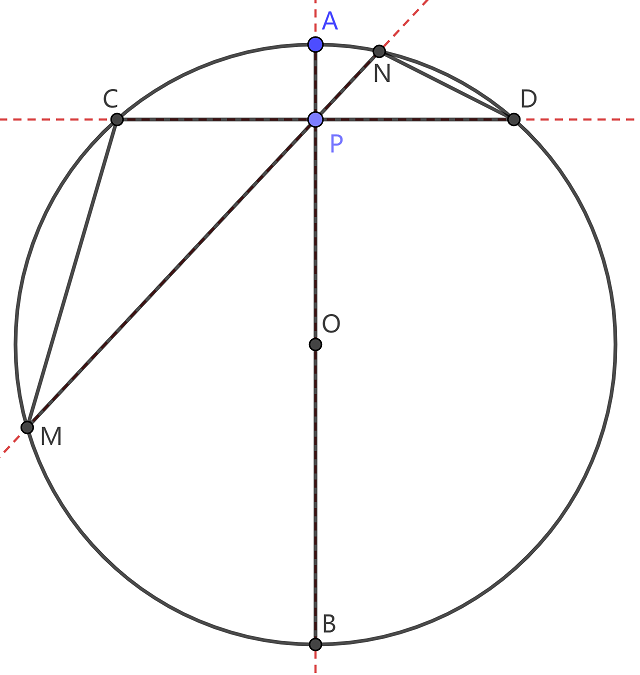
\includegraphics[width=0.42\textwidth]{圆势1.png}
\end{wrapfigure}

如右图,可以发现,$\angle NDC$和$\angle NMC$都对应同一段弧,且$C,M$都在弧外,
所以$\angle NDC = \angle NMC$。又对顶角$\angle DPN = \angle CPM$,所以
$ \triangle DPN \backsim \triangle MPC$。也就是说,
$$ \frac{|PD|}{|PN|} = \frac{|PM|}{|PC|}.$$
换句话说,$|PC| \cdot |PD| = |PN|\cdot|PM|$。

对圆内一点$P$来说,即便不知道圆心,只要过$P$作直线与圆交于两点,那么$P$到两点的距离乘积
就是它到圆的势的绝对值。

如果点在圆外,是否有类似的结论呢?我们仍然连接$OP$,直线$OP$割圆于两点:$A,B$
($A$位于$O$、$P$之间)。可以算出:
$$|PA|\cdot|PB| = (|PO| - |AO|) \cdot (|PO| + |PB|) = |OP|^2 - r^2.$$
过$P$作直线$l$和圆交于两点$M,N$,$|PM| \cdot |PN|$是否也等于$|OP|^2 - r^2$呢?

如右图,注意到$\angle BNA$和$\angle BMA$都对应半圆,所以都是直角。
三角形外角$\angle PAN = \angle ABN + \angle BNA$,而$\angle ABN$和$\angle AMN$对应同一段弧且都不在弧上,
所以$\angle ABN = \angle AMN$。于是,
$$\angle PAN = \angle ABN + 90^\circ = \angle AMN + \angle BMA = \angle BMN.$$
这说明$\triangle PAN \backsim \triangle PBM$,所以
$$ \frac{|PA|}{|PN|} = \frac{|PM|}{|PB|},$$
换句话说,$|PM|\cdot |PN| = |PA|\cdot |PB|$。
我们把这个性质总结为:

对圆内一点$P$来说,即便不知道圆心,只要过$P$作直线与圆交于两点,那么$P$到两点的距离乘积
就是它到圆的势。

因此,无论在圆内还是圆外,经过一点$P$的直线与圆交于两点,则它到两点的距离乘积只与它和圆的远近关系有关。
如果$P$在圆内,这个乘积等于$r^2 - |PO|^2$;如果$P$在圆外,这个乘积等于$|PO|^2 - r^2$。
或者说,这个乘积就是势的绝对值。至于$P$在圆上的情形,我们可以认为它与圆交于两点,其中一点就是它自身,
所以到自身距离为$0$,从而乘积总是$0$,等于它的势。

\begin{tm}\textbf{圆势定理}\label{tm:0-3-40}
    过点$P$作直线与圆$(O, r)$交于两点:$A$、$B$,那么
    $$ |PA| \cdot |PB| = \left||PO|^2 - r^2\right|. $$
\end{tm}

比起乘积$|PA| \cdot |PB|$,点到圆的势多了正负号。如何理解这个正负号呢?如果过圆$(O,r)$的圆心
作一条直线,在上面建立数轴。当我们把原点$P$选在圆内的时候,$A$和$B$就对应符号相异的数;如果
把原点$P$设在圆外,$A$和$B$就代表同号的数了。
所以,以$P$为原点,$PO$为正方向的数轴和圆交于两点,这两点代表的数的乘积就是$P$到圆的势。
或者说,圆势附带了$P$和$A$、$B$的位置关系的信息。

\section{切线}
过一点作直线要与圆交于两点不难,与圆交于一点则不简单。
根据直线交圆公理,过圆内的点,无法作和圆相切的直线。过圆外一点,可以作与圆相切的直线
直观上,我们可以把直尺从和圆相交的状态逐渐移动,直到尺子碰到圆的“边缘”,作出大致和圆相切的直线。

直线和圆相切是一种特殊的状况。过圆外或圆上一点的直线$l$如果和圆$O$相切,就说它是点到圆的\textbf{切线}。
切线和圆的(唯一)交点,称为\textbf{切点}。根据相切的性质,过圆心$O$作关于$l$的垂线,切点就是垂足。
过圆上一点,只有一条切线,过圆外一点,可以作两条切线。

过圆$(O,r)$外一点$P$作切线,记切点为$Q$,则$\triangle OQP$为直角三角形。根据勾股定理,
$$ |PQ|^2 + |OQ|^2 = |OP|^2.$$
因此,$|PQ|^2 = |OP|^2 - r^2$。也就是说,点$P$到切点的距离平方,
是它关于圆的势。若过$P$作圆$O$的割线,交圆于$A$、$B$两点,那么由上一节可知
$$ |PA| \cdot |PB| = |OP|^2 - r^2 = |PQ|^2.$$
也就是说,
$$ \frac{|PA|}{|PQ|} = \frac{|PQ|}{|PB|}.$$
因此,$\triangle PAQ \sim \triangle PQB$。这两个三角形的相似关系称为\textbf{切割线定理}。

从切割线定理可以推出:$\angle PQA = \angle PBQ$。从另一个角度,可以这样理解:
过圆上一点$Q$只有一条切线$PQ$。如果过$Q$再作一条直线,直线于圆必交于另一点$A$,
而$\angle PQA$等于圆弧$\widearc{QA}$对应的圆周角。

\chapter{圆和多边形}
我们对圆上一点、两点引出的形状都有了初步了解,现在来看圆上多个点对应的形状。

\section{三角形的外接圆和内切圆}
首先来看三个点的情形。

设$A$、$B$、$C$是圆$(O,r)$上(相异的)三点,则线段$AB$、$BC$、$AC$的垂直平分线都过圆心$O$。
因此,$O$是$\triangle ABC$的外心(这里附带说明了圆上相异三点必然不共线),$|OA|=|OB|=|OC|=r$。
反之,设有(非退化的)$\triangle ABC$,以它的外心$O$为圆心,以$|OA|$为半径,就可以画出一个圆,
过顶点$A$、$B$、$C$。这说明,\textbf{不共线的三点恰好对应一个圆}。或者说,\textbf{不共线的三点确定一个圆}。
我们把这个圆称为三角形的\textbf{外接圆}(“外心”即“外接圆圆心”的简称),把三角形称为圆的\textbf{内接三角形}。

三角形不仅可以内接于圆,圆也可以内接于三角形。考虑三角形$ABC$的内心,它到三角形三边的距离相等。
以内心为圆心,以它到三边的距离为半径作圆,这个圆和三角形三边都相切。我们把这个圆叫做三角形的\textbf{内切圆}
(“内心”即“内切圆圆心”的简称),把三角形称为圆的\textbf{外切三角形}。

除了内心,三角形还有旁心。旁心到三角形三边的距离也相等。因此,以每个旁心为圆心,以它到三遍的距离为圆心,
各可以得到一个圆。每个圆都与三角形一边和另两边的延长线相切。这三个圆称为三角形的旁切圆
(“旁心”即“旁切圆圆心”的简称),把三角形称为它们的\textbf{旁切三角形}。

\section{圆内接四边形}
在三个点的基础上再加一个点$D$,四个点$A$、$B$、$C$、$D$能否恰好对应一个圆呢?显然,
$\triangle ABC$和$\triangle BCD$的外接圆未必是同一个圆。所以,四个点不总是在同一个圆上。
换句话说,要让四个点共圆,这四个点必须满足一定的条件。

% 圆内接四边形ABCD

如右图上情形,设$A$、$B$、$C$、$D$圆$(O,r)$上(相异的)四点,考察它们对应的圆弧。我们发现,
$\widearc{ABC}$和$\widearc{CDA}$是整个圆的分划,因此,它们对应的圆心角之和是周角。
根据圆周角定理,$\angle ABC + \angle CDA = 180^\circ$。同理,$\angle BCD + \angle DAB = 180^\circ$。

我们还可以发现,圆周角$\angle BAC$和$\angle BDC$都对应$\widearc{BC}$,因此根据“等弧对等角”,
$\angle BAC = \angle BDC$。同理可得:$\angle ACB = \angle ADB$,$\angle CAD = \angle CBD$,
$\angle DBA = \angle DCA$。

% 从这些等角关系出发,
% 如果对角线$AC$和$BD$交于点$P$,那么$\triangle APB \backsim \triangle CPD$、$\triangle BPC \backsim \triangle DPA$。

如果$A$、$B$、$C$、$D$顺序改变,如右图下情形,那么四边形$ABCD$就是蝶形。
$\widearc{ABC}$和$\widearc{CDA}$对应同一段圆弧$\widearc{AC}$。
这时$\angle ABC + \angle CDA = 0^\circ$,或者说$\angle ABC = \angle ADC$。
同理,$\angle BAD = \angle BCD$。

综合两种情况,\textbf{圆内接四边形对角要么和为平角,要么相等}。

可以看到,如果把相交的对边
$AB$、$CD$看作对角线,把对角线$AC$、$BD$看作对边,我们就得到一个凸四边形$ACBD$。
因此,观察相同的圆弧对应的圆周角可以发现,我们仍然有$\angle BAC = \angle BDC$、$\angle ACB = \angle ADB$,$\angle CAD = \angle CBD$,
$\angle DBA = \angle DCA$。如果对角线$AC$和$BD$交于点$P$,仍然有$\triangle APB \backsim \triangle CPD$、$\triangle BPC \backsim \triangle DPA$。
换句话说,即便圆内接四边形不是凸四边形,用它的顶点也能画出圆内接凸四边形,并且不妨碍我们讨论相关的性质。
所以,我们总把圆内接四边形问题归结为凸四边形来讨论,也称之为四边共圆问题。

以上是圆内接四边形边和角的性质,反过来,满足什么性质的四边形是圆内接四边形呢?
或者说,满足什么条件的四个点共圆呢?

\begin{tm}\label{tm:0-3-0}
    如果凸四边形$ABCD$中的一对内角$\angle ABC$与$\angle CDA$的和是平角,
    那么$ABCD$是圆内接四边形。
\end{tm}

\begin{proof}
    $\angle ABC + \angle CDA = 180^\circ$,所以要么两个角都是直角,要么一个是钝角,一个是锐角。\\
    如果两个角都是直角,作对角线$AC$,取它的中点$O$。$\triangle ABC$是直角三角形,$AC$是斜边,
    根据直角三角形的中线定理,$|AO| = |BO| = |CO|$。同理,$\triangle CDA$是直角三角形,$AC$是斜边,
    于是$|AO| = |DO| = |CO|$。因此$A,B,C,D$四点都在$\odot_{(O, A)}$上。\\
    如果两个角一个是钝角,一个是锐角。不妨设$\angle ABC > 90^\circ > \angle CDA$。作对角线$AC$,
    则$B$、$D$在$AC$两侧。作对角线$AC$的垂直平分线$l$。
    显然,$\triangle ABC$和$\triangle CDA$的外心都在$l$上,只需证明两者是同一点。\\
    设$\triangle ABC$的外接圆为$\odot_{(O_1, B)}$。$\angle ABC$是钝角,因此它的圆心角对应优弧。
    于是,$O_1$和$B$在直线$AC$两侧。$\angle CO_1A = 360^\circ - 2\angle ABC$。\\
    另一方面,设$\triangle CDA$的外接圆为$\odot_{(O_2, D)}$。$\angle CDA$是锐角,因此它的圆心角对应劣弧。
    于是,$O_2$和$D$在直线$AC$同一侧。$\angle CO_2A = 2\angle CDA$。\\
    以上两个结论说明,$O_1$和$O_2$都和$D$在直线$AC$同一侧,且$\angle CO_1A = \angle CO_2A$。
    而$\triangle CO_1A$和$\triangle CO_2A$都是等腰三角形,所以两者同角全等。这说明$O_1$和$O_2$是同一点。
    $A,B,C,D$四点都在$\odot_{O_1, A}$上。
\end{proof}

从这个定理可以推出,矩形、等腰梯形和正方形都是圆内接四边形。

\begin{tm}\label{tm:0-3-10}
    如果凸四边形$ABCD$中,$\angle ACB = \angle ADB$,
    那么$ABCD$是圆内接四边形。
\end{tm}

\begin{proof}
    $ABCD$是凸四边形,所以$C$和$D$在直线$AB$同侧。
    作边$AB$的垂直平分线$l$,显然,$\triangle ABC$和$\triangle ABD$的外心都在$l$上,
    只需证明它们是同一点。\\
    设$\triangle ABC$的外接圆为$\odot_{(O_1, C)}$,
    $\triangle ABD$的外接圆为$\odot_{(O_2, D)}$。
    如果$\angle ACB$是钝角,那么它的圆心角对应优弧。
    于是,$O_1$和$C$在直线$AB$两侧,且$\angle BO_1A = 360^\circ - 2\angle ACB$。
    这时,$\angle ADB = \angle ACB$也是钝角,所以同样有$O_2$和$D$在直线$AB$两侧,且
    $\angle BO_2A = 360^\circ - 2\angle ADB$。
    如果$\angle ACB$是锐角,那么它的圆心角对应劣弧。
    于是,$O_1$和$C$在直线$AB$同侧,且$\angle BO_1A = 2\angle ACB$。
    这时,$\angle ADB = \angle ACB$也是锐角,所以同样有$O_2$和$D$在直线$AB$同侧,且
    $\angle BO_2A = 2\angle ADB$。\\
    因此,$O_1$和$O_2$总在直线$AB$同侧,且$\angle BO_1A = \angle BO_2A$。
    而$\triangle BO_1A$和$\triangle BO_2A$都是等腰三角形,所以两者同角全等。这说明$O_1$和$O_2$是同一点。
    $A,B,C,D$四点都在$\odot_{O_1, A}$上。
\end{proof}

\begin{tm}\label{tm:0-3-20}
    过一点$P$的两条直线$m,n$上各有两点:$A, C\in m$和$B, D \in n$,分别各在$P$两侧。
    如果
    $$ |PA| \cdot |PC| = |PB| \cdot |PD|, $$
    那么四边形$ABCD$是圆内接四边形。
\end{tm}

\begin{proof}
    考虑$\triangle APB$和$\triangle DPC$。对顶角$\angle APB = \angle DPC$。
    而$ |PA| \cdot |PC| = |PB| \cdot |PD|$等于说
    $$ \frac{|PA|}{|PB|} = \frac{|PD|}{|PC|}.$$
    因此根据“边角边”,$\triangle APB \sim \triangle DPC$。于是有
    $\angle ABP = \angle DCP$,$\angle BAP = \angle CDP$。因此,根据定理\ref{tm:0-3-10},
    四边形$ABCD$是圆内接四边形。
\end{proof}
这个定理也可以理解为:两条线段相交,如果交点把每条线段分成的两部分长度之积相等,那么线段端点共圆。
也就是说,这两条线段实际上是圆的两条相交的弦。

反之,圆的两条弦$AC$和$BD$相交于$P$,则“等弦对等角”说明$\angle ACD = \angle ABD$、
$\angle BAC = \angle BDC$。因此$\triangle ABP \sim \triangle DCP$,
$ |PA| \cdot |PC| = |PB| \cdot |PD|$。

\begin{tm}\textbf{相交弦定理}\label{tm:0-3-30}
    圆的两条弦$AC$和$BD$相交于$P$,则
    $$ |PA| \cdot |PC| = |PB| \cdot |PD|. $$
\end{tm}

\begin{xt}
    \mbox{}\\
    给定圆内接凸四边形$ABCD$。$E$是对角线$AC$上一点。$\angle CDE = \angle BDA$。\\
    \indent 1. 证明:$\triangle CDE \sim \triangle BDA$。\\
    \indent 2. 证明:$\triangle CDB \sim \triangle EDA$。\\
    \indent 3. 证明:$|AC| \cdot |BD| = |AB| \cdot |CD| + |BC| \cdot |DA|.$\\
    给定凸四边形$ABCD$,作射线$CE$使得$\angle ECD = \angle ABD$,
    作射线$DE$使得$\angle CDE = \angle BDA$。两射线交于点$E$。\\
    \indent 1. 证明:$\triangle CDE \sim \triangle BDA$。\\
    \indent 2. 证明:$\triangle CDB \sim \triangle EDA$。\\
    \indent 3. 证明:$|AC| \cdot |BD| \geqslant |AB| \cdot |CD| + |BC| \cdot |DA|.$ \\
    \indent 4. 证明,凸四边形$ABCD$是圆内接四边形,当且仅当$|AC| \cdot |BD| = |AB| \cdot |CD| + |BC| \cdot |DA|.$\\
    \indent 5. 证明:$A,B,C,D$四点共圆,当且仅当$|AC| \cdot |BD| = |AB| \cdot |CD| + |BC| \cdot |DA|.$

\end{xt}

\section{垂心组和外接圆}

\begin{wrapfigure}[5]{r}{0.5\textwidth} %this figure will be at the right
    \vspace{-90pt}
    \flushright
    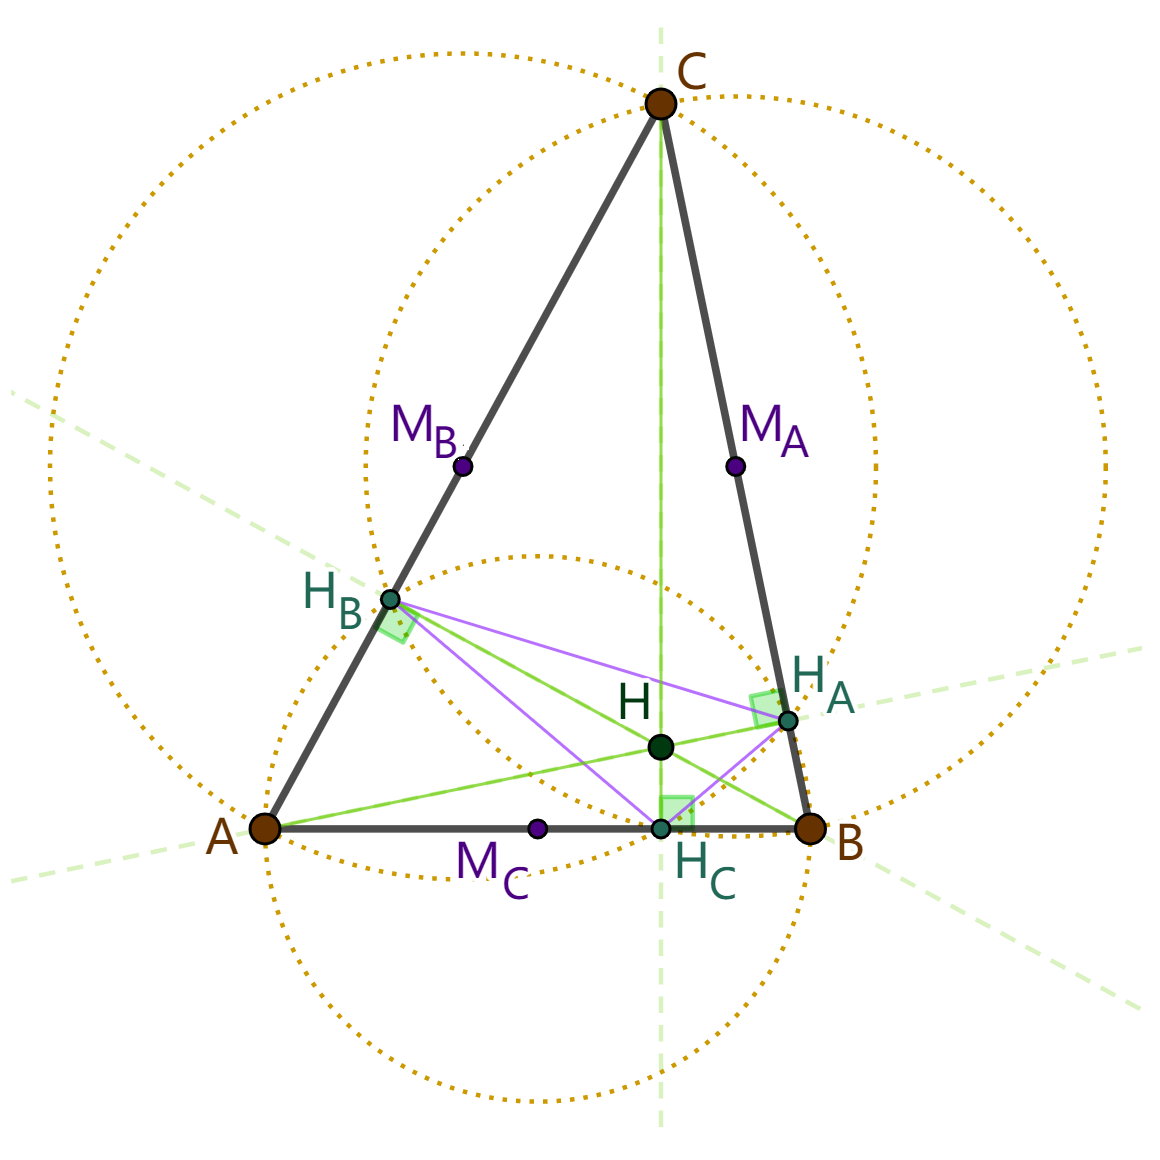
\includegraphics[width=0.48\textwidth]{垂心与外心1.png}
    \caption*{\texttt{垂心组}}
\end{wrapfigure}

考虑锐角三角形$ABC$,把顶点到对边的垂足分别记作$H_A, H_B, H_C$,垂心为$H$。
由于$\angle HH_AB = \angle BH_CH = 90^\circ$,两角之和为平角,故$H, H_A, H_C, B$四点共圆。
这说明$\angle H_CHH_A + \angle H_ABH_C = 180^\circ$。这说明$\angle CHA = \angle H_CHH_A$是钝角,
$\triangle AHC$是钝角三角形。

考察钝角三角形$AHC$,可以发现,它的顶点到对边的垂足也是$H_A, H_B, H_C$,而垂心是$B$。

类似地,我们可以证明$H, H_B, H_C, A$四点共圆,$H, H_A, H_B, C$四点共圆。
钝角三角形$BHC$、$CHA$的顶点到对边的垂足也是$H_A, H_B, H_C$,
而垂心分别是$A$和$B$。

于是,从锐角三角形$ABC$及其垂心$H$出发,可以得出四个三角形,每三个点构成的三角形的垂心,
是四个点中剩余的那个点。我们把这样的四点称为\textbf{垂心组}。

从钝角三角形及其垂心出发,一样可以得到一个垂心组。从直角三角形出发,其垂心和直角顶点重合,
四点的垂心组退化为三点。

从上面的讨论可知,垂心组四点共享三个垂足。任一顶点、垂心和另外两个顶点对应的垂足四点共圆。

考察$A, H_B, H_A, B$四点。由$\angle AH_BB = 90^\circ = \angle AH_AB$可知,
$A, H_B, H_A, B$四点共圆。由于$\angle AH_BB$是直角,$A, H_B, H_A, B$四点所在的圆,
圆心是边$AB$的中点$M_C$。同理,$A, H_C, H_A, C$四点共圆,圆心是边$AC$的中点$M_B$;
$B, H_C, H_B, C$四点共圆,圆心是边$BC$的中点$M_A$。

从$A, H_B, H_A, B$四点共圆可以推出:$\angle A = \angle CH_AH_B$,$\angle B = \angle H_AH_BC$。
也就是说,$\triangle CH_BH_A \backsim \triangle CBA$。

从以上两个四点共圆性质还可以推出$\angle HH_CH_A = \angle CAH$,$\angle HH_AH_C = \angle ACH$。
因此,$\triangle HH_AH_C \backsim \triangle HCA$。

以上是三角形垂心组的基本性质。垂心是顶点到对边垂线的交点。另外一个和边垂直的概念是边的中垂线。
如果把三角形的垂心和外心一起来看,会发现两者有密切的关联。

考虑锐角三角形$ABC$、其垂心$H$及其外心$O$。边$BC$可以看作$\triangle ABC$外接圆的弦。
圆心角$\angle BOC = 2\angle A$,因此在等腰三角形$BOC$中,
$$\angle CBO = 90^\circ - \frac{1}{2}\angle BOC = 90^\circ - \angle A = \angle HBA.$$
同理,$\angle BAO = \angle HAC$,$\angle ACO = \angle HCB$。

\begin{wrapfigure}[9]{r}{0.42\textwidth} %this figure will be at the right
    \vspace{-60pt}
    \flushright
    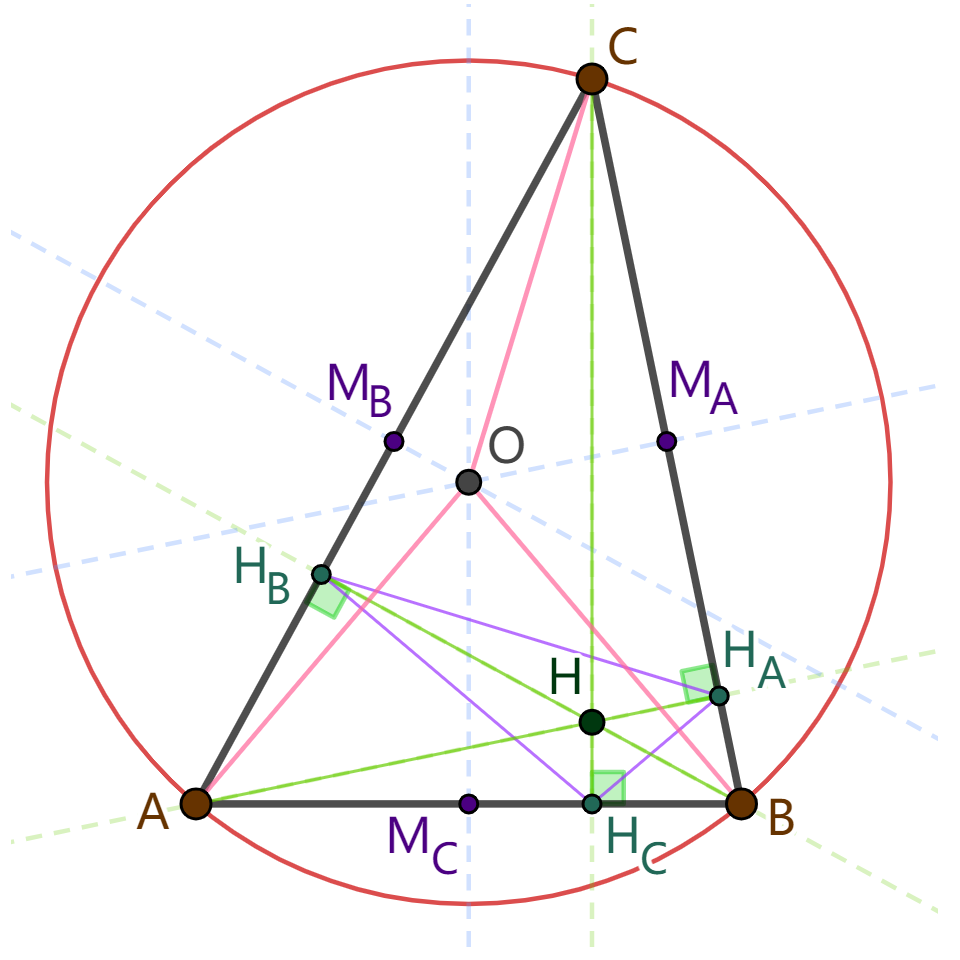
\includegraphics[width=0.4\textwidth]{垂心与外心2.png}
    % \caption*{\texttt{垂心和外接圆}}
\end{wrapfigure}

此外,$\angle H_CH_AB = \angle A$,因此$\angle H_CH_AB + \angle CBO = 90^\circ$。
这说明半径$OB \perp H_AH_C$。同理,半径$OA \perp H_BH_C$,$OC \perp H_AH_B$。

作点$A$在$ABC$外接圆上的对径点$A'$,$AA'$是直径,所以$\angle ACA'$是直角。因此
$$ \angle H_CHA' = 90^\circ - \angle ACH_C = \angle A.$$
另一方面,$A, H_B, H, H_C$四点共圆,所以
$$ \angle H_CHB = 180^\circ - \angle H_BHH_C = \angle A.$$
这说明$CA' \parallel HB$。
同理,我们可以得到$BA' \parallel HC$。因此四边形$A'BCH$是平行四边形。

作$B,C$的对径点$B', C'$,同样可以证明,
四边形$AB'HC$和$AHBC'$是平行四边形。

\begin{wrapfigure}[9]{r}{0.42\textwidth} %this figure will be at the right
    \vspace{-30pt}
    \flushright
    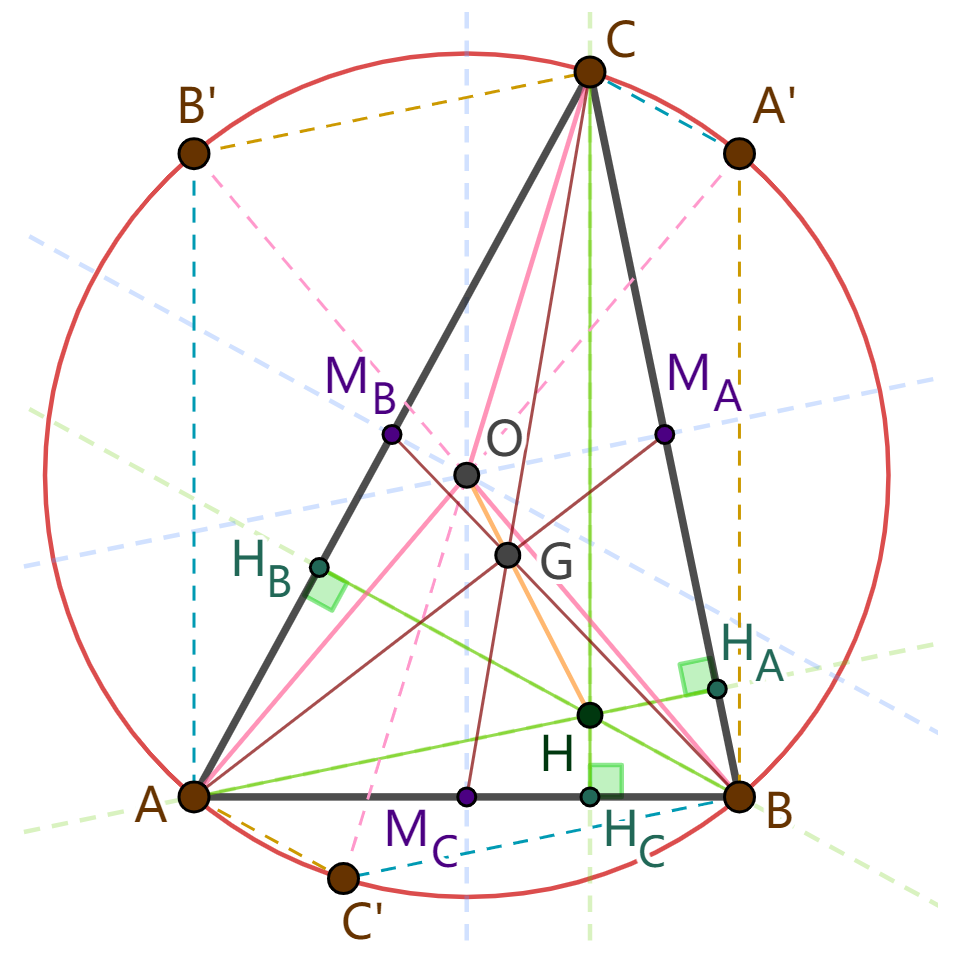
\includegraphics[width=0.4\textwidth]{垂心外心重心3.png}
    % \caption*{\texttt{垂心和外接圆}}
\end{wrapfigure}

连接圆心$O$和$AB$中点$M_C$,$O$是直径$AA'$的中点,所以$OM_C$平行于$A'B$,且长度为$A'B$一半。
我们把这种关系简称为“$OM_C$平行且等于$A'B$的一半”。

连接$OH$和$AM_C$。由于$OM_C$平行且等于$A'B$的一半,$A'B$平行且等于$HC$,
因此$OM_C$平行且等于$HC$的一半。记$OH$和$CM_C$交点为$G$,
不难看出,$\triangle OGM_C \sim \triangle GHC$,且
$$ \frac{|M_CG|}{|GC|} = \frac{|OG|}{|GH|} = \frac{|OM_C|}{|HC|} = \frac{1}{2}.$$
也就是说,点$G$在三角形$ABC$中线$CM_C$上,且到$C$点的距离是到$M_C$距离的两倍。
这说明$G$就是三角形$ABC$的重心。我们发现,三角形的垂心、外心和重心满足以下的性质:

\begin{tm}{\textbf{三心共线定理}}\label{tm:1-2-10}
    \mbox{} \\
    三角形$ABC$的垂心、外心和重心共线,重心位于外心和垂心为端点的线段上,
    而且重心到垂心的距离是重心到外心距离的两倍。
\end{tm}

\begin{xt}\label{xt:1-2-10}
    沿用本节记号,证明: \\\
    \indent 1. $|AH|\cdot |HH_A| = |BH|\cdot |HH_B| = |CH|\cdot |HH_C|.$\\
    \indent 2. $H$是$\triangle H_AH_BH_C$的内心。\\
    \indent 3. 记$\triangle ABC$的内心为$I$,旁心分别为$J_A, J_B, J_C$,则$I$是$\triangle J_AJ_BJ_C$的垂心。\\
    \indent 4. $H$关于$AB$的对称点$H^C$在$ABC$外接圆上,且$\widearc{AC'} = \widearc{H^CB}$。\\
    \indent 5. $\triangle AHB$、$\triangle AHC$和$\triangle CHB$的外接圆都和$\triangle ABC$的外接圆一样大。
    它们的圆心分别是$\triangle ABC$的外心$O$关于三边的对称点,和$O$组成垂心组。
    并且这个垂心组和垂心组$A,B,C,H$全等。
\end{xt}

\section{九点圆}

我们已经了解过三角形的外接圆、内切圆和旁切圆。本节我们再介绍三角形内部的一个特殊的圆。

设有三角形$ABC$,上一节中,我们证明了$\triangle ABC$的垂心$H$、外心$O$和重心$G$共线。
考虑线段$OH$,作它的中点$M$。我们知道$AHBC'$是平行四边形,所以$M_C$是其对角线$HC'$的中点。
因此,$MM_C$平行且等于$OC'$的一半。

作$CH$的中点$D_C$,由于$OM_C$平行且等于$CH$的一半,因此平行且等于$HD_C$。
也就是说,四边形$HD_COM_C$是平行四边形,于是$M_C, M, D_C$共线,$M$是$M_CD_C$的中点,
$|MD_C| = |MM_C| = \frac12 |M_CD_C|$。

$\triangle M_CH_CD_C$是直角三角形,所以斜边中点$M$到直角顶点$H_C$的距离是斜边长度$M_CD_C$的一半。
也就是说,
$$ |MD_C| = |MM_C| = |MH_C| = \frac12 |OC'| = \frac{\mathtt{R}}{2}.$$
其中$\mathtt{R}$是$ABC$的外接圆半径。

\begin{wrapfigure}[7]{r}{0.42\textwidth} %this figure will be at the right
    \vspace{-20pt}
    \flushright
    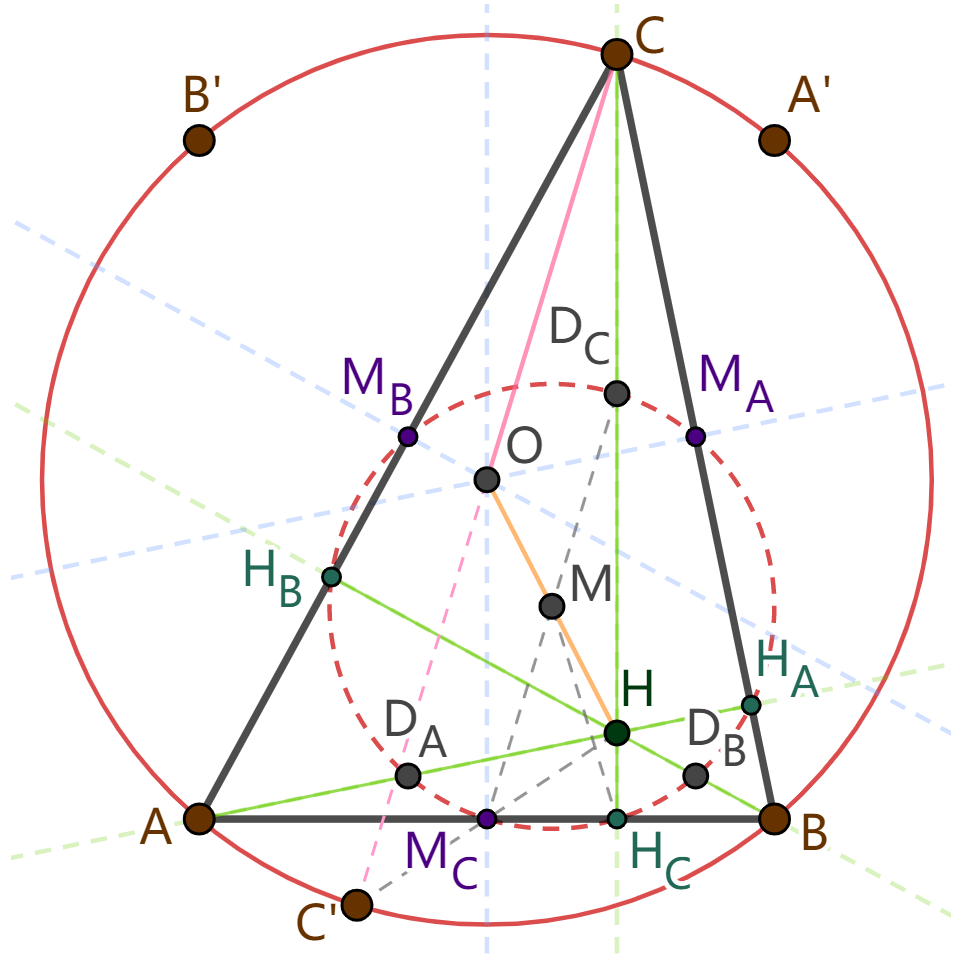
\includegraphics[width=0.4\textwidth]{九点圆1.png}
    % \caption*{\texttt{垂心和外接圆}}
\end{wrapfigure}

同理,我们也有
\begin{align}
    |MD_A| = |MM_A| = |MH_A| = \frac{\mathtt{R}}{2}, \notag \\
    |MD_B| = |MM_B| = |MH_B| = \frac{\mathtt{R}}{2} \notag 
\end{align} 
所以,以$M$为圆心,以$\frac{\mathtt{R}}{2}$为半径画圆,我们就会发现,这个圆经过三边中点,
三边上的垂足,以及三顶点到垂心连线的中点,合共九点。我们把这个圆称为\textbf{九点圆}。

\begin{tm}{\textbf{九点圆定理}}\label{tm:1-3-10}
    \mbox{} \\
    三角形三边中点、三边垂足,以及三顶点到垂心连线的中点共圆。
    圆心为外心与垂心的中点,半径为三角形外接圆半径的一半。
\end{tm}
三角形的九点圆的大小,刚好是三角形外接圆的一半。如果我们把三角形的垂心$H$看作“起点”,
那么三角形的外接圆可以看作是九点圆外延加倍得到的。比如,把线段$HD_C$加倍延长,就得到$HC$;
把线段$HM_C$加倍延长,就得到$HC'$;把线段$HH_C$加倍延长,就得到外接圆上一点$H^C$。
一般来说,从$H$出发,连接$H$和九点圆上任一点,加倍延长后,终点就会落在外接圆上。

\begin{xt}
    沿用本节记号,证明:\\
    \indent 1. 作外心$O$关于三边的对称点:$O_A, O_B, O_C$,则垂心$H$是$\triangle O_AO_BO_C$的外心。\\
    \indent 2. $\triangle O_AO_BO_C \simeq \triangle ABC$。两者关于点$M$对称,有共同的九点圆。\\
    \indent 3. 记$\triangle ABC$的旁心为$J_A, J_B, J_C$,则$\triangle J_AJ_BJ_C$的九点圆是$\triangle ABC$的外接圆。
\end{xt}

\section{圆内接多边形}
九点圆涉及了内接于同一个圆的九边形。对一般的多边形来说,成为圆内接多边形意味着什么呢?

从四边形的情况来看,顶点的位置顺序对形状很重要。如果顶点$A$、$B$、$C$、$D$按顺时针或逆时针顺序排列,
那么四边形$ABCD$是凸四边形,否则,四边形$ABCD$可能是凹四边形。

对一般的圆内接多边形,我们只研究最简单的一类:顶点按逆时针顺序排列的多边形。
具体来说,设圆$O$上有$n$个点:$A_1, A_2, \cdots , A_n$,从$A_1$出发构造圆映射$\gamma_{(O,A_1)}$,
把$[0, 360)$映射到圆周,那么$0$对应$A_1$。设$t_1, t_2, \cdots , t_n$分别对应$n$个点,
那么$0 = t_1 < t_2 < \cdots < t_n$。这样定义的圆内接多边形:$A_1A_2\cdots A_n$就是我们研究的对象。
这样定义的多边形,每个内角都在零角和平角之间。这样的多边形叫做\textbf{凸多边形}。

对于大于等于$3$的整数$n$,凸$n$边形$A_1A_2\cdots A_n$有$\frac{n(n-3)}{2}$条对角线。
具体来说,每个顶点和相邻两个顶点的连线是$n$边形的边,和其余$n-3$个顶点的连线是对角线。
因此每个点是$n-3$条对角线的端点。另一方面,每条对角线对应两个顶点,因此一共有$\frac{n(n-3)}{2}$条对角线。

凸多边形的内角和是否有规律呢?我们知道三角形的内角和是平角,凸四边形的内角和是两个平角
(或者说周角,如果把角度约定在负平角和正平角之间,则减去一个周角变成零角)。边数继续增多时,
我们定义凸$n$边形$A_1A_2\cdots A_n$的内角和为:

$$ \angle A_1A_2A_3 + \angle A_2A_3A_4 + \cdots + \angle A_{n-2}A_{n-1}A_{n} + \angle A_{n-1}A_{n}A_{1}+ \angle A_{n}A_{1}A_{2}$$

如果我们不把角度限定在负平角和正平角之间,可以猜测:凸$n$边形的内角和是$n-2$个平角。

如果凸多边形是圆内接多边形,我们可以这样证明:$n$个顶点把圆分为$n$段圆弧。每个顶点张成的内角,
对应了其中$n-2$段圆弧。如果考虑所有$n$个内角对应的圆弧,则每段圆弧计入$n-2$次(圆弧两端是内角顶点的时候不计入,
其它情况下都计入)。也就是说,$n$个内角和对应$n-2$个整圆。这些内角都是圆周角,
因此它们的和是$n-2$个整圆对应的圆周角,即$n-2$个平角。我们的猜想至少对圆内接多边形是正确的。

对一般凸多边形的情况,我们可以通过不断“裁剪”三角形来证明。我们还记得,凸四边形可以裁成两个三角形,
因此它的内角和是两个三角形的内角和。从另一个角度来看,我们通过裁掉一个三角形,把凸四边形变成了三角形。
对一般的凸$n$边形$A_1A_2\cdots A_n$来说,由于它的每个内角都介于零角和平角之间,我们可以考虑裁掉某个角,
把它变成$n-1$边形。比如,沿着线段$A_1A_3$剪一刀,
就把$A_1A_2\cdots A_n$分成了三角形$A_1A_2A_3$和$n-1$边形$A_1A_3\cdots A_n$。

\begin{tm}\label{tm:1-4-0}
    凸$n$边形的内角和是$n-2$个平角。
\end{tm}
\begin{proof}
    用归纳法证明。命题$P(n)$:凸$n+2$边形的内角和是$n$个平角。我们要证明$P(n)$对所有正整数$n$成立。\\
    $n=1$时,由于三角形内角和是平角,$P(1)$成立。\\
    假设$P(n)$成立,下面证明$P(n+1)$成立。\\
    设有凸$n+3$边形$A_1A_2A_3\cdots A_n$,将它裁成三角形$A_1A_2A_3$和$n-1$边形$A_1A_3\cdots A_n$。
    前者的内角和是平角。根据$P(n)$,后者的内角和是$n$个平角,因此,$A_1A_2A_3\cdots A_n$的内角和是$n+1$个平角。
    于是$P(n+1)$成立。\\
    因此对所有正整数$n$,命题$P(n)$成立。
\end{proof}

满足什么条件时,凸多边形是圆内接多边形呢?最直接的条件,自然是平面上有一个圆,
使多边形顶点都在圆上。或者说,能找到一点,到多边形各个顶点距离相等。

如果难以直接找到这样的点,可以查看多边形各边和各条对角线的垂直平分线。
如果多边形是圆内接多边形,它的边和对角线都是圆的弦,垂径定理说明其垂直平分线过圆心。
具体来说,可以考察两条边(或对角线)的垂直平分线的交点。这点如果到各个顶点距离相等,
那么多边形内接于以它为圆心的圆,否则多边形不是圆内接多边形。

有一种特殊的凸多边形必然是圆内接多边形:\textbf{正多边形}。
正多边形是各边等长,各内角相等的多边形。正三角形、正方形都是正多边形。
正多边形各个的内角角度是$\frac{180(n-2)}{n}^\circ$。

\begin{xt}\label{xt:1-4-0}
    \mbox{}\\
    \indent 1. 平行四边形、矩形、正方形、梯形、筝形,哪些总是圆内接多边形?哪些可以是圆内接多边形?要满足什么条件?\\
    \indent 2. 设有整数$1 \leqslant i,j,k,l \leqslant n$,圆内接$n$边形$A_1A_2\cdots A_n$中,$\angle A_iA_kA_j$和$\angle A_iA_lA_j$有什么关系?
\end{xt}

% \section{弧长和面积}
% 直观上,我们知道圆和圆弧的形状。我们已经学过,半径为$r$的圆,面积是$\pi r^2$,周长是$2\pi r$。
% 其中的$\pi$是常数,叫圆周率,大约等于$3.14$。在公理体系中,如何证明这一点呢?

% 这些知识看似不难,但要从基本的定义和公理出发,得到


\chapter{三角函数}
通过研究点、直线、角和三角形、四边形、圆形,我们对简单的平面图形有了更多的认识。
其中对三角形的研究贯通了我们对各种形状的探索。通过对三角形性质的理解,
我们建立了三角形和四边形、圆形乃至更复杂的形状之间的关系。

如果对前面学习的知识做一次整理,我们会发现,大多数的结论要么和共点、共线、共圆有关,
要么是长度之间、角度之间的相等或简单倍数关系。我们把这些结论称为定性结论。

在科学研究和生产实践中,我们更需要知道的是形状之间定量的关系。
比如,如果三角形的三边长度分别是$4,5,6$,我们希望知道三角形内角到底是多少度。
又比如,如果菱形两条邻边长度为$1$,夹角为$50^\circ$,我们希望知道菱形对角线的长度。

为了研究形状之间的定量关系,我们仍然从三角形开始研究。

\section{正弦函数}
如右图,我们想知道三角形$ABC$中$\angle B$的角度和对边$AC$长度的关系。
为此,我们作$ABC$的外接圆$O$,则$AC$是$O$的弦。$\angle B$作为圆周角,是圆心角$\angle COA$的一半。
作$AC$中点$M$,则$\angle B = \angle MOA$。再假设外接圆半径为$1$,
我们就把一般三角形的边角关系转化成了特定直角三角形的边角关系。

反过来,假设我们知道了斜边长度为$1$的直角三角形中,直角边和对角的关系,
我们就能知道外接圆半径为$1$时,三角形内角和对边的关系。
对于一般的三角形,只要按照外接圆半径的比例放大或缩小成$1$,就可以知道边和对角的关系了。

那么,直角三角形的角和边有什么关系呢?我们先来看另一个问题。

考虑半径为$1$的圆$O$(这样的圆以后常常遇到,我们把它叫做\textbf{单位圆}),连接圆心$O$和圆上两点,
就构成一个三角形。为了方便讨论,我们以其中一点为“起点”,另一点为“终点”。设起点所在的直径是“水平”的,
而终点在圆上其他位置(如下图)。

\begin{figure}[H] %this figure will be at the right
    \vspace{4pt}
    \centering
    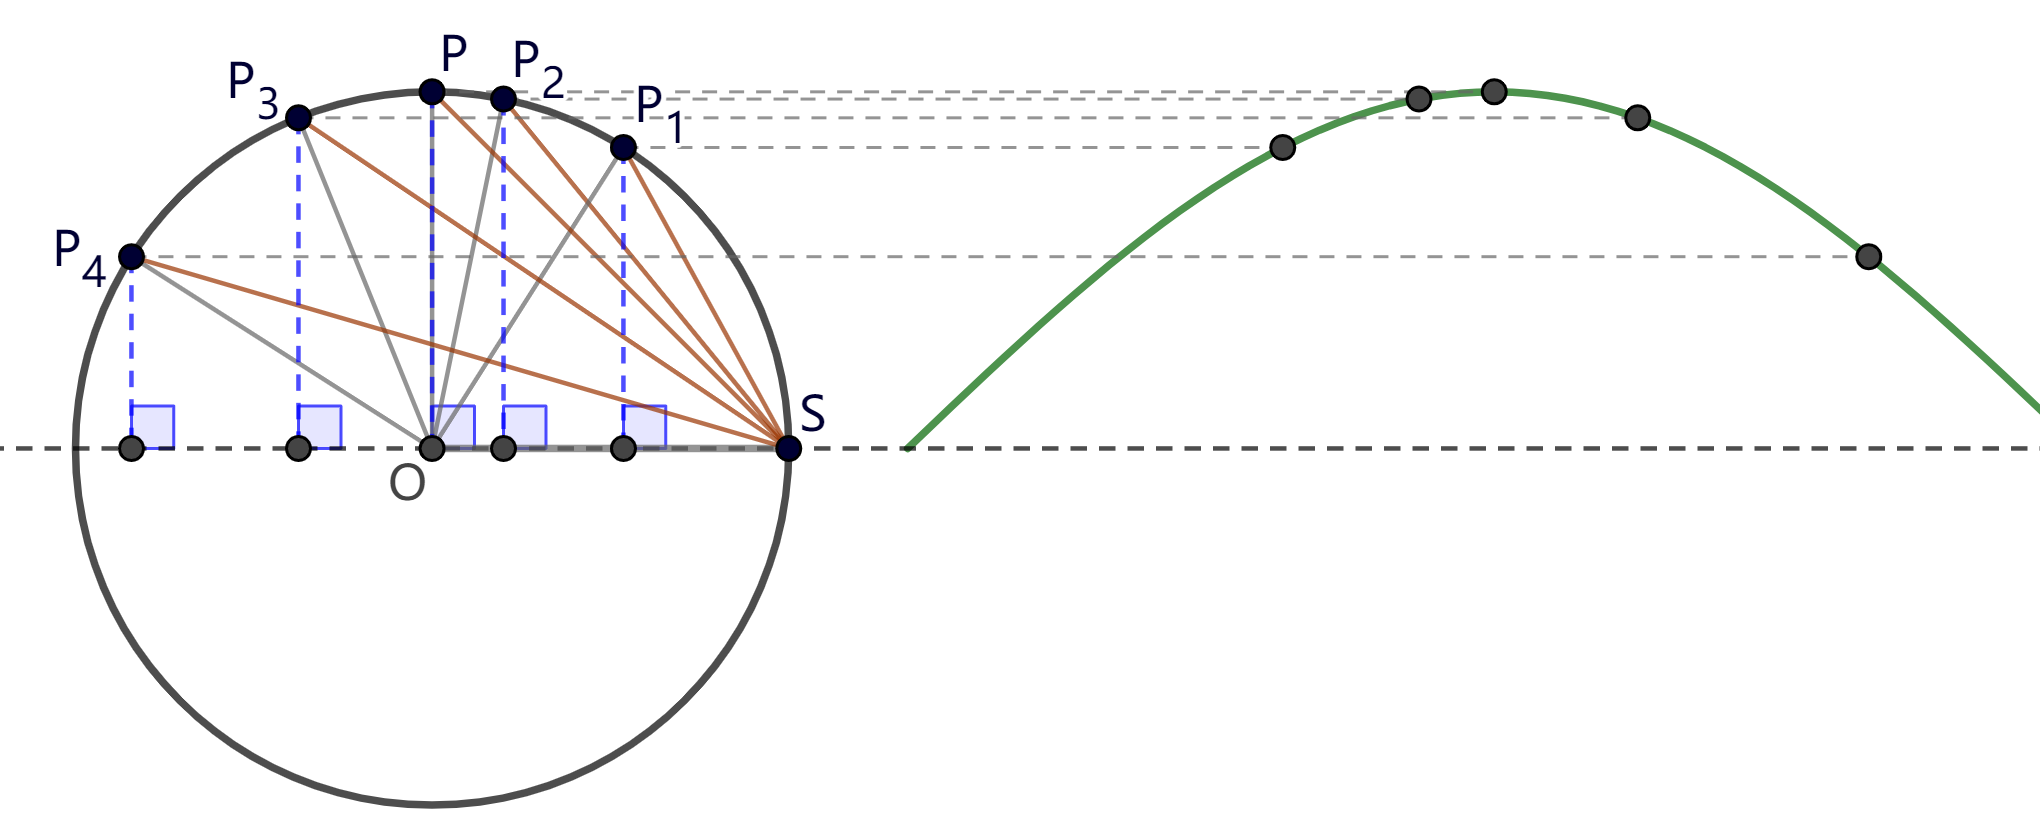
\includegraphics[width=0.8\textwidth]{三角函数2.png}
    % \caption*{\texttt{垂心和外接圆}}
\end{figure}

\section{余弦函数}
\section{三角函数和三角形}
\section{正切和余切函数}


\chapter{从或许到确定}
预测未来,是人类社会的重要活动。合理有效地预测未来,是社会文明进步的标志。
中华文明作为农耕文明,很早就懂得预测未来的重要性。
历法、史书、节气,都是我们的祖先为了后人更好地预测未来,留下的经验总结。

生产活动中,预测尤其重要。比如,农牧业、渔业、运输业等行业需要预测天气,
销售行业需要预测产品的市场需求。科学研究和工程制造中,如果能够提前知道产品在各种各样的情境和场景下的性能,
可以节约大量人力物力。社会要发展,就需要更高的预测水平。

\section{事件和见知}

如何判断某件事情将来会不会发生?我们要依赖已有的知识和经验。日常生活中,
我们会说“明天大概要下雨”、“今年冬天肯定很冷”、“我明天大概去不了了”。根据已有条件,
有些事情必然发生,有些事情或许会发生,有些事情不可能发生。事情发生与否,取决于某些条件。
我们把这样的事情叫作\textbf{随机事件},简称\textbf{事件}。
在已知条件下,如果某事件必然发生,就说它是\textbf{必然事件};
如果某事件必然不发生,就说它是\textbf{不可能事件};
如果某事件或许会发生,就说它是\textbf{或然事件}。数学中,研究这些事情的理论叫作概率论。

概率论假定,我们关心的随机事件有某些恒定的内在规律,受某些固有未知因素的影响。
概率论通过研究这些内在规律和因素,预测事件是否会发生。

如何描述一个事件?从客观的角度,我们可以把“发生一件事”看成事物状态、形势局面的改变。
一件事是否发生,可以用改变后的状态或局面表示。我们也许无法确定未来事物发展成哪个状态、形势走向哪个局面,
但我们可以事先确定事物未来所有可能的状态、所有可能出现的局面。

比如,我们无法确定明天杭州是否下雨,但我们知道,在明天杭州是否下雨这个问题上,只可能出现两个结局:下雨或不下雨。
又比如,我们投一个骰子前,无法确定朝上一面的点数,但我们知道,投出的骰子最终只有六个状态:
朝上一面是$1,2,3,4,5$或$6$点。这些最终状态、局面是\textbf{互斥}的。比如明天杭州不可能既下雨又不下雨,
骰子停下之后不可能既是$1$点朝上又是$2$点朝上。

我们把所有可能的最终状态或局面看成一个集合,集合中的每个元素称为事情的\textbf{终态}或\textbf{结局}。
比如,考虑明天杭州是否下雨这个问题时,所有结局构成$\{\mbox{下雨}, \mbox{不下雨}\}$这个集合,
每次投骰子时,骰子的终态构成$\{1,2,3,4,5,6\}$这个集合。我们把这个集合叫作\textbf{终集},即终态的全集。
我们可以把相关的事件用终集的子集表示。比如,“明天杭州下雨”对应$\{\mbox{下雨}\}$这个子集,
“骰子点数是偶数”对应$\{2,4,6\}$这个子集。事物发展的终态如果在子集里,就说明事件发生了,否则事件没有发生。

单元集也对应着事件。我们把这些事件叫做\textbf{基本事件}。
不是任何其他事件的交集的事件,叫做基本事件。比如$\{1\}$对应的“骰子点数是$1$”就是基本事件。
基本事件是各种事件的“基本单元”,它们通过合并形成别的事件。基本事件之间是互斥事件,它们是终集的分划。

终集可以是有限的,也可以是无限的。目前我们只讨论有限的情况。
要注意的是,随着问题的条件、环境、思考问题的角度发生变化,终集也会变化。
比如,我们考虑明天杭州下雨的问题时,可能要把准备经过杭州的台风“凤凰”也考虑在内。
台风“凤凰”也许继续靠近,也许转向。这时,我们的终集是:
$$\{\mbox{台风靠近且下雨}, \mbox{台风靠近且不下雨}, \mbox{台风转向且下雨}, \mbox{台风转向且不下雨}\}$$

而“明天杭州下雨”对应子集$\{\mbox{台风靠近且下雨}, \mbox{台风转向且下雨}\}$。

对于随机事件,如果我们知道得更多,就能作出更准确的预测。
比如,如果我们不知道台风的情况,那么即便我们把终集依照“台风是否继续靠近”划分,
我们能把握的也只是$\{\mbox{台风靠近且下雨}, \mbox{台风转向且下雨}\}$、
$\{\mbox{台风靠近且不下雨}, \mbox{台风转向且不下雨}\}$两个事件,
与$\{\mbox{下雨}\}, \{\mbox{不下雨}\}$并没有不同。
如果我们掌握了台风的动向,我们就希望把$\{\mbox{下雨}\}$分成\\   
$\{\mbox{台风靠近且下雨}\}$和$\{\mbox{台风转向且下雨}\}$来讨论了。
可以说,随着我们对事物、形势的认知增加,我们的终集会越来越“细”。

为了描述认知增加的过程,我们从最“细”的终集出发,定义每个阶段的\textbf{知集},代替不同阶段的终集。
知集是最“细”终集的子集构成的集合,满足:

\begin{enumerate}
    \item 空集属于知集;
    \item 如果集合$A$属于知集,那么$A$的补集也属于知集;
    \item 如果集合$A$和$B$属于知集,那么它们的并集也属于知集。
\end{enumerate}

知集表示我们每个阶段的认知。我们根据当前的认知来讨论各种事件。
比如,在杭州下雨的例子里,可以有两个知集,分别是:
$$ S_1 = \big\{\varnothing, \{\mbox{AR}, \mbox{DR}\},\{\mbox{AN}, \mbox{DN}\}, \{\mbox{AR}, \mbox{AN}, \mbox{DR}, \mbox{DN}\} \big\}$$

和
\begin{align}
    S_2 &= \big\{ \varnothing, \{\mbox{AR}\}, \{\mbox{AN}\}, \{\mbox{DR}\}, \{\mbox{DN}\}, \{\mbox{AR}, \mbox{AN}\}, \{\mbox{AR}, \mbox{DR}\}, \{\mbox{AR}, \mbox{DN}\}, \notag \\
    & \{\mbox{AN}, \mbox{DR}\}, \{\mbox{DN}, \mbox{AN}\}, \{\mbox{DR}, \mbox{DN}\},  \{\mbox{AR}, \mbox{AN}, \mbox{DR}\}, \{\mbox{AR}, \mbox{AN}, \mbox{DN}\}, \notag \\
    &  \{\mbox{AR}, \mbox{DR}, \mbox{DN}\},  \{\mbox{AN}, \mbox{DR}, \mbox{DN}\}, \{\mbox{AR}, \mbox{AN}, \mbox{DR}, \mbox{DN}\} \big\} \notag 
\end{align}
其中$\mbox{AR}, \mbox{AN}, \mbox{DR}, \mbox{DN}$分别表示
“台风靠近且下雨”、“台风靠近且不下雨”、“台风转向且下雨”和”台风转向且不下雨“。
可以看出,$S_1$是$S_2$的子集。$S_1$到$S_2$的过程,就是对台风认知加深的过程。

这种描述下,不同的知集就对应不同“粗细”的终集。每个知集都对应自己的基本事件。
这时候的基本事件不一定是单元集。比如,$\{\mbox{AR}, \mbox{DR}\}$在$S_1$中是基本事件,在$S_2$中就不是基本事件了。

\begin{xt}
    写出以下问题的终集和知集。\\
    \indent 1. 我国朱鹮从东北省份向南迁徙的路线有三条:西线、中线和东北线。
    小明想知道黑龙江省的某只朱鹮沿哪条路线南迁。\\
    \indent 2. 某航空公司规定:作为补偿,飞机晚点一小时以上,返还全票票价的$40\%$;
    如果晚点三小时以上,返还全票票价的$75\%$。乘客实际购票价低于前述返还价格的,
    返还乘客实际购票价。航班因晚点取消,且乘客自愿接受转乘下一班机的,公司协助补票,
    实施“就低返利”政策:按照下一班机实时票价和乘客最初购票价的较低者计算新票价,多则退还差价;
    并另外补偿新票价的$30\%$。某乘客购票后,在候机时被告知飞机可能晚点,他试着分析可能得到的晚点补偿。
\end{xt}

\section{概率和分布}

预测随机事件时,我们除了关心会发生什么事情,还关心事情有多大可能发生。
当我们说“这事百分之百能成”,“他八成还在路上”,“他的话只有三分准头”,
我们认为某些事情比另一些事情更可能发生。习惯上,我们用数来描述事情有多大可能发生。
在数学中,我们把这个做法称为\textbf{事件的概率}。

我们用不大于$1$的非负实数表示事件的概率。约定不可能事件的概率是$0$,必然事件的概率是$1$。
事件的概率越大,越有可能发生。
此外,事件的概率应当和事件之间的关系相符。两个互斥事件同时发生的概率应该是$0$,
至少有一个发生的概率应该是它俩概率的和。用集合的语言来说,空集的概率应该是$0$,
终集的概率应该是$1$;两个集合不相交,那么它们的并集的概率等于它们概率的和。

我们习惯用映射$\mathbb{P}$来记录概率。把事件$A$的概率记为$\mathbb{P}(A)$。
比如,我们说明天八成会下雨,可以写成$\mathbb{P}(\{\mbox{下雨}\}) = 0.8$。
不至于混淆时,也可以省略表示集合的大括号,写成:$\mathbb{P}(\mbox{下雨}) = 0.8$。

基本事件两两互斥,并集是终集(全集)。所以,基本事件的概率之和等于$1$。

举例来说,投骰子的时候,我们一般认为投出$1,2,3,4,5,6$点的可能性都一样大,
即每个基本事件的概率都相等。于是它们各自的概率是六分之一。
据此,可以算出任何事件的概率。比如,“投出$5$点或以上”的概率是“投出$5$点”的概率加上“投出$6$点”的概率,
也就是三分之一。如果我们知道骰子有问题,比如投出$6$点的可能性是其他任一点数的$2$倍,
那么“投出$6$点”的概率是七分之二;投出其他点数,比如“投出$3$点”的概率是七分之一;
而“投出$5$点或以上”的概率是七分之三。

终集是有限集合的时候,对每个知集来说,只要知道了其中每个基本事件分配到的概率(称为\textbf{概率分布}),
就可以推出知集里其他事件的概率。

\begin{sk}
    同一个终集下的不同知集中,同一个事件的概率是否相同?
\end{sk}

\section{二项分布和均匀分布}

我们来看两种简单的概率分布。

考虑只有两个终态$a, b$的终集,两个基本事件$\{a\}, \{b\}$概率之和是$1$。
设其中一个的概率是$p$,则另一个的概率是$1-p$。我们把这样的概率分布叫作\textbf{二项分布}。
举例来说,如果我们认为明天杭州下雨的概率是$0.7$,不下雨的概率就是$1-0.7=0.3$。
我们说,我们认为明天杭州下雨的问题服从二项分布。

又比如:抛一枚硬币,我们认为正面朝上的概率是$0.52$,那么反面朝上的概率就是$1 - 0.52 = 0.48$。
我们说,我们认为抛这枚硬币的问题服从二项分布。
为了好说话,我们会在两个基本事件中选一个我们更关心的,称为\textbf{正面事件},把另一个称作\textbf{反面事件}。
如果正面事件的概率是$p$,就说问题服从系数为$p$的二项分布。

终集为$\{a, b\}$的二项分布,包括四个事件,分别对应$\varnothing, \{a\}, \{b\}, \{a, b\}$四个子集。
设$\{a\}$是正面事件,概率为$p$,那么这四个事件的概率分别是$0$、$p$、$1-p$和$1$。

对于元素更多的终集,情况更加复杂。我们考虑一种简单情形:每个基本事件的概率相等。
这样的概率分布称为\textbf{等概率分布}或\textbf{均匀分布}。
比如,投骰子时,如果我们认为每面朝上的概率都相等,就说投骰子服从均匀分布。

假设终集有$n$个终态,那么每个基本事件的概率就是$\frac{1}{n}$。
对于任意事件,我们可以数一下事件包含了几个终态,用终态个数除以所有终态的个数,
就是它的概率。我们把这个性质写作:
$$ \mathbb{P}(A) = \frac{|A|}{|S|} $$
其中$|A|$表示事件$A$作为集合的元素个数,$|S|$表示终集$S$的元素个数。 
比如,服从均匀分布的投骰子问题中,要求“大于$2$点”的概率,我们数一下事件$\{3,4,5,6\}$,
它包含了$4$个终态,所以“大于$2$点”的概率是$4 \times \frac{1}{6} = \frac{2}{3}$。

\begin{xt}
    \mbox{} \\
    \indent 1. 把$1$到$100$分别写在小纸条上放入黑箱里,随意抽取一张,
    抽到的数是素数的概率是多少?完全平方数的概率是多少?各位数字乘积大于$10$的概率是多少? \\
    \indent 2. 有没有以全体自然数为终集的均匀分布?为什么?说说你的理由。
\end{xt}

% \section{条件概率和独立事件}
% 讨论随机事件,总要知道前提条件。只有明确了前提条件,才能讨论事件的概率。
% 为了研究不同的前提条件对事件的影响,我们引入条件概率的概念。

% 仍以“明天杭州是否下雨”为例。我们讨论台风“凤凰”动向对下雨概率的影响,可以说:
% “如果台风靠近,那么下雨的概率有$90\%$”、“如果台风转向,那么不下雨的概率为$40\%$”。
% 这里我们把台风靠近与否作为明天杭州下雨的前提条件。以上两句话可以记作:
% $$ \mathbb{P} (\{\mbox{下雨}\} \, | \, \{\mbox{台风靠近}\}) = 0.9, \quad \mathbb{P} (\{\mbox{不下雨}\} \, | \, \{\mbox{台风转向}\}) = 0.4$$
% 从知集$S_2$的角度,$\mathbb{P} (\{\mbox{下雨}\} \, | \, \{\mbox{台风靠近}\}$应该记为:
% $$  \mathbb{P} (\{\mbox{台风靠近且下雨}, \mbox{台风转向且下雨}\} \, | \, \{\mbox{台风靠近}\}$$
% 但我们知道,在“台风靠近”的前提条件下,

\section{排列和组合}
均匀分布的问题里,事件的概率只和它包含的终态的个数以及所有终态的个数有关。因此,在相关的一些问题里,
我们关心如何计出事件包含的终态的个数。

\begin{ex}
    将编号为$1,2,3$的$3$个小球排成一列,最左边的球是$1$的概率是多少?
\end{ex}
要知道事件“最左边的球是$1$”的概率,用“最左边的球是$1$”包含的终态个数除以所有终态的个数。
怎么计算“最左边的球是$1$”包含的终态个数和所有终态的个数呢?

首先考虑所有终态的个数:将编号为$1,2,3$的$3$个小球排成一列,有多少种方法?

不妨设三个球从左到右排列。无论排列方式如何,三个球分别占据“左”、“中”、“右”三个位置。
从左边开始,把球一个个放到位置上。左边的位置可以放三个球中任何一个,因此有$3$种方法。
按任一种方法放好左边的球以后,中间的位置可以放剩余两个球中任何一个,因此有$2$种方法。
按任一种方法放好中间的球以后,右边的位置可以放最后一个球,只有$1$种方法。
于是一共有$3\times 2\times 1 = 6$种方法。

如果最左边的球是$1$,有多少种方法?这时左边的位置已经放好了$1$号球,因此中间的位置还有两种放法。
任一种方法放好中间的球以后,右边的位置放最后一个球,只有$1$中方法。因此,一共有$2\times 1 = 2$种方法。

综上所述,“最左边的球是$1$”的概率是:
$$ \mathbb{P}(\mbox{最左边的球是}1) = \frac{2}{6} = \frac{1}{3}. $$

我们把$n$个互不相同的物品排成一列的方法数目称为$n$\textbf{排列数},记作$P_n$。
比如,编号为$1,2,3$的$3$个小球排成一列的方法数目就叫做“$3$排列数”,记作$P_3$。

对于一般的自然数$n$,$n$排列数是$n-1$排列数的$n$倍。
这是因为,如果把$n$个互不相同的物品排成一列,第一个位置总可以放$n$个物品中的任何一个,
有$n$种方法。按任一种方法放好第一个位置后,剩下的$n-1$个位置摆放剩下的$n-1$个物品的方法数目,
恰好就是$n-1$排列数。

因此,用归纳法可以证明,$n$排列数就是$n$乘以$n-1$乘以$n-2$……直到乘以$1$的乘积。比如,
$5$排列数就是$5\times 4\times 3\times 2\times 1 = 120$。

如果我们把从$n$乘到$1$的计算看成关于$n$的函数的话,这个函数叫做($n$的)\textbf{阶乘},记作$n!$。
$n$排列数就是$n$的阶乘。

\begin{ex}
    将$3$个红球和$2$个白球组成一列,最左边的球是红球的概率是多少?
\end{ex}
我们仍然先计算$3$个红球和$2$个白球组成一列的方法数。
这里球只有红白两种颜色的分别。同色的球没有差别。如果我们把球编号,$1,2,3$号球是红球,$4,5$号球是白球,
那么,按照编号排列,有$5! = 120$种方法。不过,$1-2-3-4-5$和$2-3-1-4-5$其实是同一种方法。
因为$1,2,3$号球都是红球,并没有差别。把$1-2-3-4-5$里的$3$个红球任意改变次序,都不影响结果。同理,
把$1-2-3-4-5$里的$2$个白球任意改变次序,都不影响结果。$3$个红球的排列方法有$3! = 6$种,$2$个
白球的排列方法有$2! = 2$种,于是这$6\times 2 = 12$种方法都对应同一种结果。也就是说,带编号的$12$个排列方法
对应一种不带编号的排列方法。因此,实际上只有$\frac{5!}{3!2!} = 10$种排列方法。

我们把不带编号的排列方法称为\textbf{组合数}或\textbf{选列数}。
比如,$3$个红球和$2$个白球组成一列的方法数目叫做“$3,2$组合数”,或“$5$选$3$”
(因为也可以看作从$5$个位置里选$3$个放红球),记作$C_5^3$或$5 \choose 3$。

如果最左边的球是红球,那么剩下的$4$个位置要放$2$个红球、$2$个白球。于是,一共有$C_4^2$种方法。计算可知:
$$ C_4^2 = \frac{4!}{2!\times 2!} = \frac{24}{2\times 2} = 6.$$
即一共有$6$种方法。因此最左边的球是红球的概率是:
$$ \mathbb{P}(\mbox{最左边的球是红球}) = \frac{C_4^2}{C_5^3} = \frac{6}{10} = \frac{3}{5}.$$

一般来说,“$n$选$m$”也可以用阶乘计算:
$$ C_n^m = \frac{n!}{m!(n-m)!} $$

容易发现:“$n$选$m$”等于“$n$选$n-m$”。比如,$5$选$3$等于$5$选$2$。
用红球和白球的例子,可以理解为:$3$个红球和$2$个白球组成一列的方法数目,
等于$3$个白球和$2$个红球组成一列的方法数目。

掌握了排列数和组合数,我们就可以计算一些复杂问题里终态的个数。

\begin{xt}
    \mbox{} \\
    \indent 1. $5$个红球和$3$个白球排成一列,有多少种方法?\\
    \indent 2. $2$个红球、$3$个白球和$2$个黄球排成一列,有多少种方法?\\
    \indent 3. 从编号$1,2,3,4,5$的$5$个球中选出$3$个排成一列,有多少种方法?这个数目叫做$5,3$排列数。
    试求一般情况下$n,m$排列数(从编号为$1$到$n$的$n$个球中选出$m$个排成一列的方法数目)的公式。\\
    \indent 4. 设有两个正整数$m < n$,证明:$m!$整除$n!$。
\end{xt}

% \chapter{三段论(上)}
% \begin{ex}
%     判断以下的说法对不对。\\
%     \indent 1. 哺乳动物都是恒温动物。家兔是哺乳动物。所以家兔是恒温动物。\\
%     \indent 2. 八年级有些同学没有按规定请假。至少有一个参加足球培训的同学是八年级的。
%     所以至少有一个参加足球培训的同学没有按规定请假。
%     \indent 3. 任意奇数的平方除以$8$余$1$。某整数的平方除以$8$不余$1$。
% \end{ex}
% \section{大前提、小前提和结论}
% \section{直言三段论}

\end{document}